

\section{Implementation}
We introduce the architecture of event based workflow system and then discussed the details for every component. Figure 3 shows the architecture of  event driven workflow and it's work procedure.

\begin{figure} 
\centering
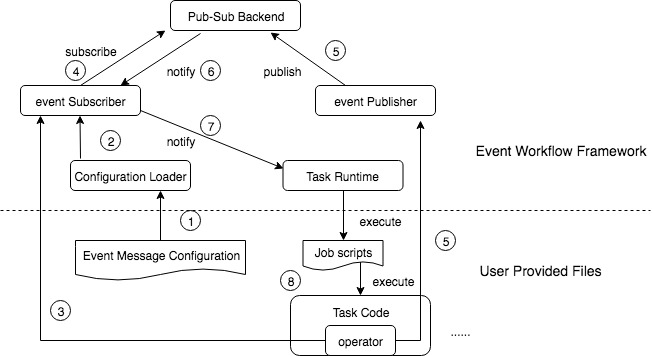
\includegraphics[width=.8\linewidth]{./figure/edflowarchitecture.jpg}
\caption{event driven workflow framework archetecture}
 \label{fg:state}
\end{figure} 


The user view and the workflow frame view are shown in Figure 3,  User need to provide the initial configuration file which define the path of the job script and the event  that every task interested, those events will be subscribed into the event store. Operator is the in-situ part integrated into the simulation code which is used to send subscribe and publish request during simulation running.   When specific events is published , the subscribe end will be notified and the job scripts will be started by task runtime. We will introduce the key component for the following parts. 


\subsection{Optimised Pub-Sub Backend}

In this part, we introduce the design and implementation of optimised pub-sub mechanism to support both traditional and in-situ task dependency patten in workflow.

Two key algorithms for event published subscribed. We leverage the canonical pub-sub mechanism and make it support the fan-in and fan-out pattern at the same time, namely one event message could subscribed multiple sub event message and specify the triggering conditions. When the all the events are published specific times, the subscribed events will be triggered subsequently.


 \begin{algorithm}
 \caption{Algorithm for event Subscribe}
 \begin{algorithmic}[1]
 \renewcommand{\algorithmicrequire}{\textbf{Input:}}
 \renewcommand{\algorithmicensure}{\textbf{Output:}}
 \REQUIRE 
 Event List (EL), subtoClientMap(event, set(clientid) , clienttoSubMap(clientid, EventPublishTimeMap(event, publishedTimes))
 \ENSURE  subscribeStatus
 \FOR {event in EL}
  \IF {key clientId exist in clienttoSubMap}
  \STATE clienttoSubMap[clientId][event]=0
  \ELSE
  \STATE init EventPublishTimeMap[event]=0
  \STATE clienttoSubMap[clientId]=EventPublishTimeMap
  \ENDIF


  \IF{key event in subtoClientMap}
   \STATE subtoClientMap[event].insert(clientId)
  \ELSE
   \STATE init set s and insert clientId
   \STATE subtoClientMap[event]=s
  \ENDIF

 \ENDFOR

 \RETURN subscribeOk
 \end{algorithmic} 
 \end{algorithm}



\subsection{Data Operator}


\subsection{Task Runtime}



/////////////old stuff////////////////////

The design and implementation details are presented in this section.
\subsection{Dynamic Task Manager of Event Workflow}
The typical event driven mechanism works based on the observe pattern, the subject component will maintain a list of observer component, if the state of the subject component changed, the notify function will send to the associated observer components. We define and optimize our task manage based on this observe pattern, specifically, every task manager could be the subject and object component at the same time, different task could compose a workflow chain and even be organized into more complex workflow. Every task manager could be create/updated/deleted dynamically during the process of the system running. User could create/update/deleted the description file of the task manager and the instance of the task manager will be changed correspondingly.


Three abstraction: TaskManager, Communicator, Operator.

\subsection{Event messages monitoring}
Event could be divided into following parts according to the event sources:
Runtime level events which created by the runtime of the tasks such as, TaskStart, TaskFail, TaskFinish.
Taskelvel which is created by tasks during the task running in fine granularity such as TimeStepWrittingFinihs or DataProcessing Finish.
Third party events, the events could be customized by users, when data satisfy specific logic, the event could be generated and pushed.
Other platform events such as DiskFull or other events related to the running of the workflow tasks.
\subsection{Event actions aggregation and matching}
\subsection{Event message generating}

\section{Evaluation and Experiments}
For traditional application, just describe the solution and evaluate the typical five pattern: latency time, 

For in-situ, using an experiments and several evaluation


\subsection{System Performance and Scalability}
1) Event latency experiments. This experiments measures the scalability of (PTT) time between event published and task triggering. 

we use synthetic application pairs to test this scalability.


The graph shows the results of the experiments, with the increasing of the application pairs:

the latency show what tendency?

what is the maximum number of clients/events that the system can support?

\subsection{Effectiveness in Scientific applications}
For this part we verify the effectiveness for our workflow engine in two different types of scientific applications according to the dynamics of the dependency. The dependency of the first type of application is already fixed before workflow running, our work flow engine could support the typical five task organization pattern \cite{todo} for this scenario. The second type is in-situ and in-transit workflow with dynamic dependency construction. The time of when the dependency is constructed depends on the properties of intermediate data during the tasks running.
